\newpage{}

\begin{center}
  \Large{\textbf{ПРИЛОЖЕНИЕ А}}\\
  \normalsize (справочное) \\ \textbf{Алгоритм защиты программы}
\end{center}
\addcontentsline{toc}{section}{Приложение А Алгоритм защиты программы}
\label{AppendixA}

\begin{figure}[h!]
  \centering
  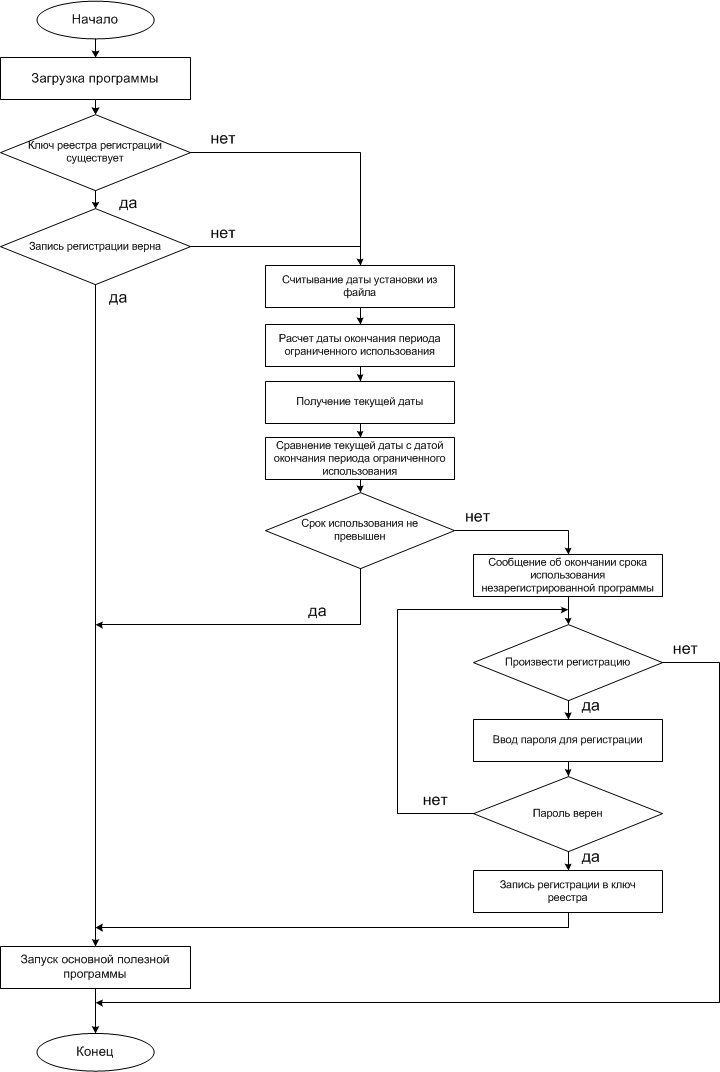
\includegraphics[height = 0.8 \textheight, keepaspectratio]{alg}
\end{figure}
\begin{center}
  Рисунок А.1 --- Алгоритм защиты программы
\end{center}

\newpage{}



%%% Local Variables: 
%%% mode: latex
%%% TeX-master: "../TermWork_PASIOB"
%%% End: 
